\chapter{Design}

\epigraph{"The longer you wait before fixing a bug, the costlier it is to fix.”}{\textit{Joel Spolsky, StackOverflow founder}}

%delete justify
\begin{flushleft}
\end{flushleft}
Il design è un aspetto fondamentale nella realizzazione della soluzione: grazie a questa fase, molti problemi sono evitati in fase di sviluppo. Il tempo impiegato in fase di design, inoltre, permette di risparmiare tempo nelle fasi successive, evitando di arenarsi contro un problema non definito a priori e non contemplato ad alto livello, per poi dover tornare indietro alla definizione del problema e rimodellare una soluzione.\\
Di seguito si descrive innanzitutto la struttura del Sistema di Warehouse, in seguito le API realizzate, e, infine, la presa in carico delle richieste.\footnote{Per rispettare le linee guida del team di sviluppo, i termini, le tecnologie impiegate ed il codice prodotto sono scritti in inglese, salvo casi eccezionali: nel corso della stesura della relazione si è mantenuto questa direttiva, per poter avere un raffronto simmetrico con il lavoro prodotto.}

\section{Warehouse} \label{warehousedesign}

Il Sistema di Warehouse deve occuparsi principalmente di due mansioni:
\begin{enumerate}
    \item Memorizzare i dati inviati dai sensori.
    \item Soddisfare le richieste degli utenti.
\end{enumerate}
La memorizzazione dei dati, prima delle mansioni, non è un aspetto innovativo del sistema, in quanto il compito era svolto anche in precedenza (si veda \ref{previousarch}). Uno degli obiettivi del nuovo sistema coincide però con la risoluzione della principale criticità riscontrata: il Database. Innanzitutto, i dati di interesse dei i sensori sono salvati in principalmente tre tabelle: 
\begin{itemize}
    \item \textbf{devices}
    \item \textbf{devices\_extras}
    \item \textbf{devlog}
\end{itemize}
Un'ottimizzazione per lo scopo finale prevede la creazione di una tabella per ognuno degli attributi registrati dai device. In più, i dati registrati sono dati di tipo time-series (dove, per time-series, si intendono quei dati che rappresentano come un sistema, processo o comportamento cambia nel tempo \cite{timescaledb})\footnote{In lingua originale: \textit{Time-series data is data that collectively represents how a system, process, or behavior changes over time.} }: una grande miglioria sarebbe inserirli all'interno di un Database con una particolare accortezza per questi dati. La scelta è ricaduta su TimescaleDB.
\paragraph{Perché TimescaleDB} TimescaleDB è pensato appositamente per i dati time-series. Si appoggia su PostgreSQL ed ottimizza il modo in cui si interrogano, accedono ed inseriscono i dati grazie, principalmente, alle \textit{Hypertables}. Per comprendere pienamente cosa rappresenta una Hypertable è prima necessario capire come TimescaleDB organizza i dati: i dati di una singola tabella sono memorizzati in sub-tabelle, chiamate \textit{chunk}, identificabili da una coppia di parametri \textbf{CHUNK\_SIZE} e \textbf{CHUNK\_TIME}, ovvero la dimensione del chunk e l'istante di tempo in cui è stato creato. Ogni sub-tabella rappresenta quindi una porzione della tabella nella sua interezza. Con TimescaleDB è possibile creare una Hypertable sulla tabella originale (la Figura \ref{fig:hypertableconcept} mostra una schematizzazione di una Hypertable), 
\begin{wrapfigure}{r}{0.40\textwidth}
    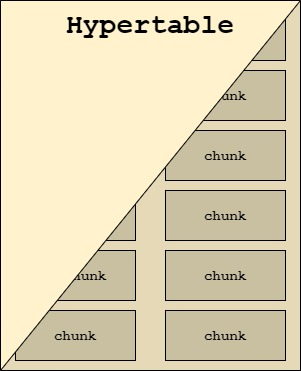
\includegraphics[scale=0.52]{images/hypertableconcept.jpg}
    \caption{Hypertable}
    \label{fig:hypertableconcept}
\end{wrapfigure}
che gestisce le operazioni nei chunk basandosi sull'attributo time che ogni tabella su cui si vuole creare una hypertable deve avere. 
In base al valore di time dell'elemento che si vuole inserire o prelevare nel Database, la hypertable seleziona il chunk in cui inserirlo o prelevarlo. Ciò rende più veloci le operazioni sui time-series data \cite{timescaledbperformance}. Un altro aspetto cruciale consiste nell'introduzione di un layer ulteriore tra il Broker MQTT ed il Database: eventuali modifiche architetturali (ad esempio il cambiamento del Database) con un nuovo strato non si propagherebbero su tutta la struttura. Il sistema di comunicazione tra BrokerMQTT e TimescaleDB è \textbf{NSQ}, di cui si discuterà in maggior dettaglio nei paragrafi successivi. \\ \\
La seconda delle mansioni del sistema vede protagonista gli utenti, e, in particolar modo, le loro richieste di ottenimento di determinati dati.\\
Deve esistere una componente del sistema che accetta ed indirizza le richieste degli end user. Questa componente è un server API, il \textit{WarehouseAPIServer}. \\
Uno dei compiti del WarehouseAPIServer prevede l'interazione con il lato del processing delle richieste, un worker, denominato \textit{WarehouseBackendWorker}, che estragga il contenuto di ciascuna di esse e le soddisfi. Poiché, per quanto già asserito in \ref{moledati}, il soddisfacimento della richiesta sarà effettuato in modo asincrono, il WarehouseAPIServer ed il WarehouseBackendWorker non possono comunicare direttamente, pena lo sviluppo di un sistema altrimenti sincrono o non correttamente sviluppato. Si vede la necessità di introdurre un elemento che si faccia carico di memorizzare e fornire le richieste.\\
Uno strumento efficace per la realizzazione di questa componente è NSQ \cite{nsqurl}. 

\paragraph{Perché NSQ} NSQ è un progetto Open Source per la distribuzione realtime di messaggi, altamente scalabile orizzontalmente e distribuito \cite{nsqfeat}. Un aspetto molto importante per il Sistema di Warehouse che NSQ offre è la consegna di un messaggio \textbf{almeno} una volta \cite{nsqfeat}: in caso di errori interni al server, una richiesta valida, invece che tornare in uno stato di errore, può essere reinserita all'interno di NSQ per poi essere riprocessata. In più, la scalabilità che offre è un punto chiave per poter ampliare, eventualmente, il sistema in futuro. Per comprendere meglio il lavoro in seguito descritto, si introducono brevemente le componenti e la logica di NSQ. NSQ si compone di 3 \textit{daemon} (processi che vengono eseguiti in background): 
\begin{itemize}
    \item nsqd, il deamon che riceve, mette in coda ed invia i messaggi. I messaggi sono inviati presso dei \textit{Topic}, i quali sono suddivisi in più \textit{Channel}.
    \item nsqlookupd, il daemon che mantiene informazioni topologiche del sistema, che ne agevola lo scaling. 
    \item nsqadmin, il daemon che fornisce un'interfaccia web per gestire la coda.
\end{itemize}
Inoltre, due ruoli chiave sono individuati: il \textbf{Producer}, che produce le informazioni ed i messaggi, ed il \textbf{Consumer}, che, di contro, li utilizza.\footnote{Nel Sistema di Warehouse, il Producer si rispecchia nel WarehouseAPIServer, mentre il consumer nel WarehouseBackendWorker.} Il meccanismo di interazione tra tutte le componenti è semplice: il Producer invia un messaggio ad un topic di nsqd. Internamente, nsqd invia una copia del messaggio a tutti i channel relativi a quel topic. Il consumer può o essere direttamente iscritto ad un channel, oppure collegarsi ad nsqlookupd, che gli invierà costantemente degli aggiornamenti su messaggi ed altro. Il daemon nsqadmin, invece, è utilizzabile per tenere traccia di tutto, ed è ovviamente opzionale per il funzionamento di NSQ. Si riporta in Figura \ref{fig:nsq} il funzionamento di NSQ nella sua configurazione più semplice.
\begin{figure}[h!]
    \centering
    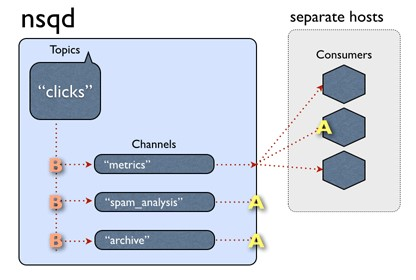
\includegraphics[scale=0.84]{images/nsq.jpg}
    \caption{Funzionamento di NSQ}
    \label{fig:nsq}
\end{figure}\\ \\
Approfondendo il WarehouseBackendWorker, componente su cui ci si è concentrati principalmente nell'ambito del lavoro svolto, esso ha un ruolo chiave nel sistema: comunica con molte delle componenti presenti, dovendo estrarre richieste da NSQ, interrogare e relazionarsi con TimescaleDB, costruire i file nei vari formati disponibili e renderli accessibili all'utente. Invece che inviare direttamente il file, tuttavia, se ne è preferita la memorizzazione su un servizio di storage, \textbf{MinIO}, a cui gli utenti potranno accedere per scaricare i risultati richiesti. Inoltre, per permettere agli utenti di sapere quando i risultati sono pronti, si è pensato ad un \textbf{Sistema di Notifiche} con cui il WarehouseBackendWorker deve interagire una volta terminata l'elaborazione di ciascuna richiesta. Come meccanismo di notifica si sono scelti inizialmente il servizio di messaggistica \textbf{Telegram} \cite{telegram}, data la sua enorme diffusione e la possibilità di configurare degli utenti automatizzati, i \textit{Bot}, per l'invio effettivo dei messaggi, ed il servizio di posta elettronica. Ciò non toglie che, in futuro, possano essere aggiunti altri mezzi di notifiche, motivo per cui il sistema deve essere sviluppato rendendo l'estensibilità di tali servizi possibile.

\paragraph{Perché MinIO} MinIO è un servizio di storage S3 compatibile \cite{miniourl}. SeismoCloud lo utilizza già per altri sistemi e servizi, per cui la sua validità è già stata provata sul campo. Per evitare problemi di spazio, legati alla dimensione dei risultati, si è stabilito che essi verranno inseriti in un archivio \textbf{ZIP} \cite{zip}, formato di compressione dei file senza perdita di dati.\\ \\ 
L'architettura per il Sistema di Warehouse che ne risulta è mostrata nella sua totalità nella Figura \ref{fig:warehousearch}.
\begin{figure}
    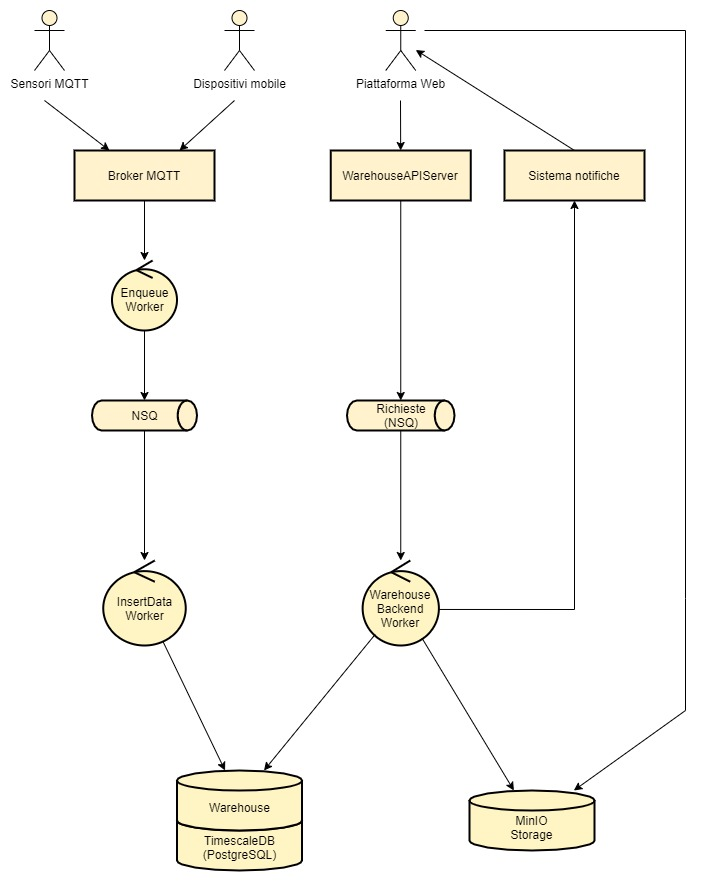
\includegraphics[left, scale=0.63]{images/warehousearch.jpg}
    \caption{Architettura del Sistema di Warehouse}
    \label{fig:warehousearch}
\end{figure}

\clearpage
\section{API}

Le API (Application Programming Interface) sono utilizzate in SeismoCloud (così come in ogni altra applicazione mobile e web) per rendere disponibili delle funzionalità agli utenti e per fungere da tramite tra layer differenti del sistema. Per consentire agli utenti di sfruttare il sistema, sono state progettate delle API che permettano un ampio accesso ai dati, secondo un cablaggio di determinati parametri da effettuare a priori dall'utente tramite la formulazione della richiesta. In SeismoCloud, le API sono progettate secondo lo stile architetturale REST (\textit{Representational State Transfer}). La loro progettazione è stata svolta in un lavoro congiunto con altri due elementi del team di sviluppo, Daniele Gargano e Igor Provornyy; esse verranno solamente accennate, in quanto il vero focus del lavoro effettuato è sul Back End del sistema e non sull'implementazione delle stesse, trattata dal primo dei collaboratori nominati.

\paragraph{Le API progettate} Come già introdotto nel capitolo precedente, le API progettate sono asincrone: l'utente, formulando una richiesta (tramite URL), non otterrà come risposta i risultati, bensì un \textbf{token} che rappresenta l'identificativo della richiesta appena effettuata. Il token gli sarà successivamente utile per controllare lo stato della richiesta, che, nel caso in cui essa sia stata processata correttamente, mostrerà l'URL alla risorsa da scaricare, altrimenti un messaggio in cui gli verrà comunicato chiaramente che la richiesta è ancora in fase di elaborazione.
\begin{wrapfigure}{l}{0.55\textwidth}
    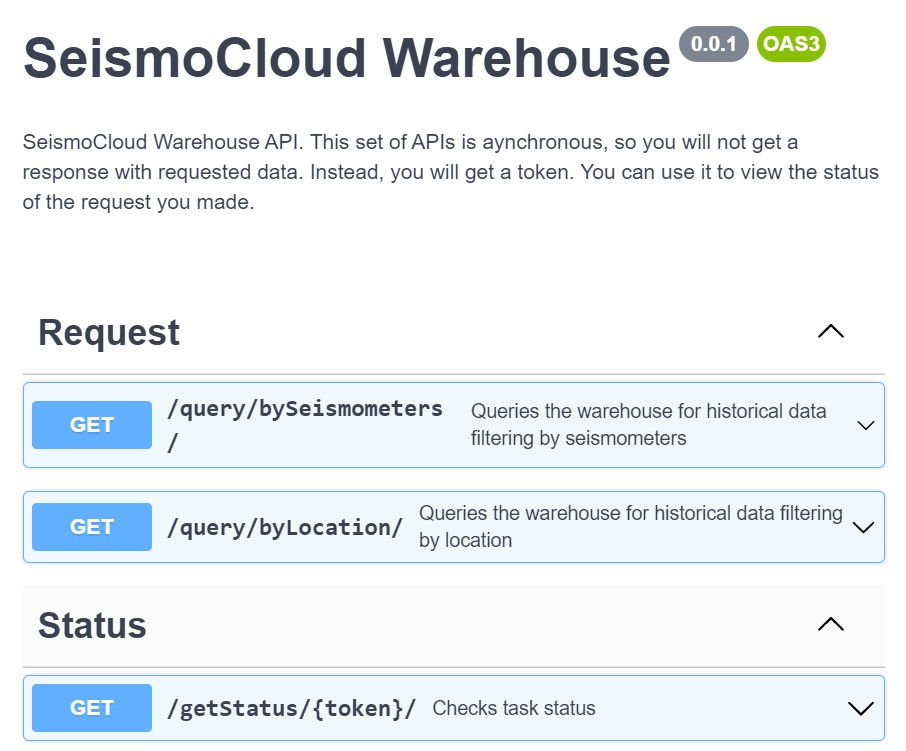
\includegraphics[scale=0.31]{images/openapi.jpg}
    \caption{Pagina web della documentazione}
    \label{fig:apiswagger}
\end{wrapfigure}
Scendendo nel dettaglio, per la scrittura e documentazione delle API si è aderito alla specifica \textbf{OpenAPI} \cite{openapi}, una specifica per la scrittura dei file per la progettazione delle API REST di tipo \textit{machine-readable format}, interpretabili dal computer. I vantaggi di questa adesione sono molteplici, dalla generazione automatica di codice alla semplicità di creazione di documentazione, come nel caso di SeismoCloud. La Figura \ref{fig:apiswagger} mostra, per l'appunto, una pagina web il cui codice HTML è stato generato automaticamente e contenente la documentazione delle API ideate.\\
I punti di congiunzione tra il Front End ed il Back End del Sistema di Warehouse sono gli \textit{endpoint} sotto il percorso \textit{/query/}: è qui che l'utente può richiedere l'accesso alle risorse, indicando i valori desiderati per i parametri quali: l'attributo o gli attributi da richiedere, che sono gli stessi trattati in \ref{apidatistorici}, la data iniziale e la data finale entro cui cercare i dati, il formato del file in cui saranno inseriti i risultati ed il metodo di ricerca, ovvero ricerca tramite identificativi dei Sismometri\footnote{fino ad un massimo di 50.} oppure tramite area geografica, identificata da una coppia di coordinate (latitudine, longitudine) ed un raggio di estensione in cui rilevare i dati. Si noti che questi due metodi di ricerca sono distinti e mutuamente esclusivi, intuibile dalla presenza dei due \textit{endpoint} \textit{/bySeismometers/} e \textit{byLocation/}. In caso di richiesta correttamente formulata, viene inviato un JSON contentente il token relativo alla richiesta. Per quanto concerne \textit{/getStatus/{token}/}, l'\textit{endpoint} permette di conoscere lo status della richiesta tramite il token fornito in precedenza.

\paragraph{Il formato del messaggio di richiesta} \label{messageformat}
Per interpretare a più basso livello la richiesta, deve essere definito un messaggio che NSQ sia in grado di leggere.
Il messaggio, sia dovendo transitare per NSQ, anello di contatto fisico tra la parte Front End e Back End del sistema, sia per uno scambio di informazioni omogeneo tra queste due componenti, necessita di un formato ben preciso e concordato tra le parti, un contratto che affermi che quanto inserito dal Producer sarà letto dal Consumer.
Il protocollo di NSQ non pone limitazioni sul tipo di dato da inserire nella coda, chiedendo che in input ci sia un array di byte, derivabile codificando secondo il formato che si preferisce; si è quindi scelto di impiegare la notazione JSON per la facile leggibilità sia lato uomo che lato macchina. Un esempio di un possibile messaggio di richiesta è nel codice sorgente \ref{code:messagejson}.
\begin{listing}[h!]
\inputminted[baselinestretch=0.8]{json}{sources/message.json}
\caption{Il messaggio espresso sotto forma della notazione JSON}
\label{code:messagejson}
\end{listing}
Si noti come il messaggio abbia al suo interno ogni elemento di cui si è precedentemente discusso, come gli \textit{Attributes} dei sismometri, quali \textit{Temperature}, \textit{RSSI}, etc., il loro \textit{ID}, la \textit{Location} desiderata\footnote{Sebbene le due informazioni facciano parte di richieste mutuamente esclusive, si è stabilito di produrre un unico messaggio ed inserire come valore di default, in caso di una richiesta \textit{bySeismometers}, il valore 0 ai campi della Location, e, viceversa, una lista vuota in caso della richiesta \textit{byDevices}}, gli handler per \textit{Telegram} e l'\textit{E-mail}, e via discorrendo. Si è inoltre aggiunto un \textit{Timestamp} per riconoscere se una richiesta è recente o meno.

\section{Gestione delle richieste} 

Per gestione delle richieste si intende tutta la serie di operazioni da effettuare nel momento in cui si deve estrarre un messaggio (che modella una richiesta) da NSQ. 
Come già accennato in precedenza, questo compito è demandato ad una componente del sistema chiamata \textbf{WarehouseBackendWorker}, parte integrante nonché principale del lavoro svolto. Il suo nome evoca la mansione che deve svolgere nel sistema: implementare il lato Back End del Sistema di Warehouse. Nello specifico, seguendo un iter che parte proprio dall'estrazione del messaggio, i passi che deve compiere sono:
\begin{enumerate}
    \item Estrarre il messaggio.
    \item Decodificare il messaggio.
    \item Interrogare il Database.
    \item Inserire i risultati nei file, rispettando il formato specificato nella richiesta.
    \item Creare un archivio nel formato \textbf{ZIP} dei file.
    \item Inserire i dati in MinIO.
    \item Notificare l'utente della disponibilità dei risultati.
\end{enumerate}
Nella Figura \ref{fig:workerflow} si schematizza il processo in maniera simile utilizzando un \textit{Activity Diagram}. Come è possibile notare, ogni passo è critico e potenzialmente potrebbe rappresentare un problema per l'effettiva elaborazione di ogni messaggio: in molti casi, in presenza di un errore, la scelta necessaria è la terminazione della richiesta. Di seguito si analizza, step by step, il compito del worker, evidenziando gli errori in cui si prevede possa incappare in questo livello di progettazione. I passi che sono enumerati rispettano le macro sequenze individuate nell'elenco precedente.
\begin{figure}[h!]
    \centering
    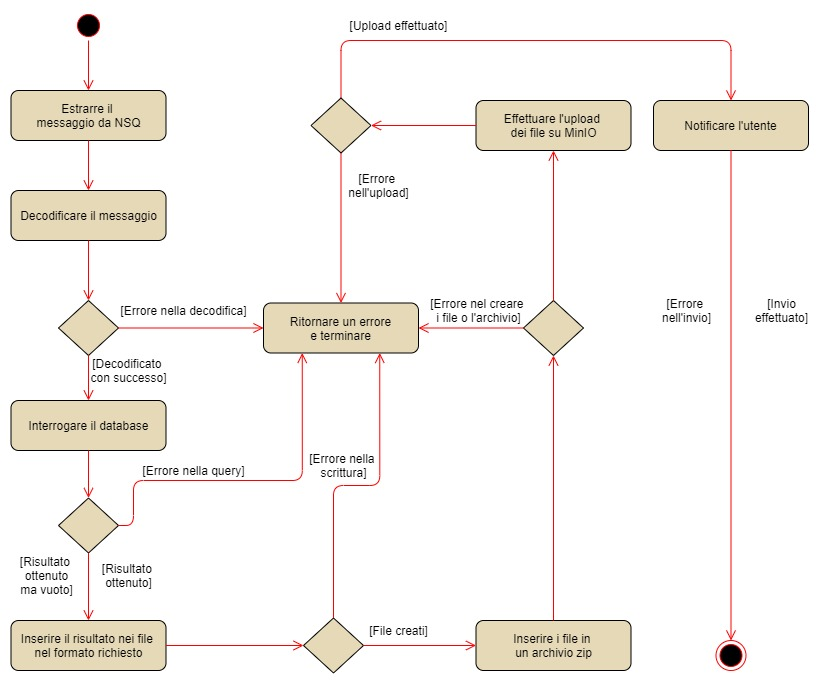
\includegraphics[scale=0.52]{images/workerflow3.jpg}
    \caption{Compiti che il WarehouseBackendWorker deve eseguire.}
    \label{fig:workerflow}
\end{figure}
\begin{enumerate}
    \item Il messaggio è direttamente inviato dall'istanza di NSQd a cui il WarehouseBackendWorker è collegato, per cui l'estrazione del messaggio non risulta avere problemi interni. Esternamente, il \textit{daemon} NSQd potrebbe andare offline, ma il problema non tange direttamente lo scopo o la rilevazione di errori del worker: il messaggio semplicemente non verrebbe recapitato.
    \item Il messaggio deve essere decodificato. Si è già dissertato sul formato che esso ha in \ref{messageformat}, per cui sarà impiegato un decoder che riesca a riprodurre il messaggio originale a partire dall'array di byte, in cui esso è espresso per il transito in NSQ. Questa decodifica potrebbe essere fallimentare, sia per una cattiva formulazione della richiesta sia per un problema inaspettato nella decodifica. In caso di entrambe le situazioni, il messaggio non può e non deve proseguire il suo ciclo vitale, ma deve essere scartato ed il worker, provvisto di un meccanismo di logging, deve comunicare il problema e ritornarlo.
    \item Il messaggio porta con sé una serie di parametri. Questi parametri sono i dati di partenza per la formulazione della/e interrogazione/i. Interrogando il Database, l'outcome atteso prevede che i risultati siano disponibili in una qualche struttura dati. Il Database potrebbe tuttavia non essere online, motivo per cui l'interrogazione fallirà, non potendo soddisfare la richiesta; potrebbe inoltre incontrare un problema internamente; oltre ciò, il risultato potrebbe essere vuoto, caso limite sulla scelta dell'azione da intraprendere successivamente. Nei primi due casi, il worker attesta l'accaduto su di un log, e lo ritorna sotto forma di errore; nell'ultimo caso, si è deciso di lasciar proseguire il lavoro, affinché l'utente possa raffrontare che quanto richiesto non ha portato a nulla, comunicandogli implicitamente che sottomettere di nuovo la richiesta non porterebbe che ad un altro file vuoto.
    \item I risultati dell'interrogazione devono essere scritti all'interno di uno o più file nel formato richiesto. Se nella scrittura ci si imbatte in un errore, il worker deve registrarlo e ritornarlo.
    \item I file devono essere inseriti in un archivio ZIP. La creazione e l'inserimento potrebbero entrambi essere problematici, per cui, anche in questo caso, il worker deve scrivere in un log il problema e ritornarlo.
    \item Deve essere effettuato l'upload dell'archivio su MinIO. Anche questa componente, così come il Database, porta con sé determinate problematiche legate alla sua disponibilità al momento della necessità: se essa non risulta disponibile, il worker non può proseguire il lavoro, non riuscendo a fornire l'output della propria esecuzione. L'upload, per citare una possibilità, potrebbe fallire, ad esempio per la caduta della connessione nel mentre. In ognuno dei casi citati l'errore va registrato e riportato, non ultimando le istruzioni.
    \item Effettuato l'upload, l'utente deve poter essere notificato. Questo passo risulta essere il più semplice, in quanto la decisione presa in caso di errori è completamente trasparente rispetto alla corretta terminazione del worker: i file sono stati correttamente inseriti, dunque disponibili. La richiesta non ha visto intoppi nella propria esecuzione. In più, il meccanismo della notifica è un optional offerto all'utente, non una condizione necessaria per l'ultimazione del lavoro: esiste un \textit{endpoint} apposito per conoscere lo status della richiesta, \textit{/getStatus/}. 
\end{enumerate}
In tutti quei casi in cui l'errore è riconosciuto come interno al server, sarebbe scorretto scartare il messaggio: potrebbero essere eliminati messaggi la cui richiesta sarebbe stata soddisfatta in casi normali. I messaggi che fanno parte di questo sottoinsieme sono dunque reinseriti in coda per essere riprocessati, per un numero ragionevole di volte.

\paragraph{Ottimizzazioni} Osservando il numero di operazioni che il \textit{WarehouseBackendWorker} deve effettuare, e considerando quanto potrebbe impiegare una richiesta, è doveroso cercare di ottimizzare il tempo di esecuzione dei singoli compiti, ove possibile. Un primo aspetto, che, in realtà, coinvolge direttamente la richiesta, è stabilire una deadline all'esecuzione di un job relativo ad un messaggio, affinché sia evitato il problema che, per qualche motivo, esso induca il worker a processarlo all'infinito, rischiando di mandare offline il server su cui esso è installato, in caso, ad esempio, di apertura continua di risorse e della loro mancata chiusura. Un secondo aspetto coinvolge il luogo di memorizzazione dei file che si stanno creando per essere caricati su MinIO: costruire un archivio ZIP per ogni richiesta, al fine di risparmiare spazio, ma mantenere i file appena creati in locale non ha una sua logica intrinseca. Una risoluzione potrebbe prevedere la creazione di una routine che ripulisca la memoria dai file obsoleti, creati a causa di richieste precedenti; un altro aspetto, forse migliore, prevede la creazione di questi file come temporanei, demandando al sistema operativo sottostante al server la gestione automatica, nonché l'eliminazione, di questi file. Come si vedrà nel capitolo \ref{implementazione}, sono state eseguite differenti iterazioni per rendere il più efficiente possibile questa operazione.

